\documentclass[conference]{IEEEtran}
\IEEEoverridecommandlockouts
\usepackage{cite}
\usepackage{amsmath,amssymb}
\usepackage{graphicx}
\usepackage{booktabs}
\usepackage{tikz}
\usetikzlibrary{arrows.meta}
\usepackage{textcomp}
\graphicspath{{figures/}}

\begin{document}

\title{Early-Warning Fall Prediction from Wearable Sensors:\\
A Cost-Sensitive, Time-to-Impact Trade-off Analysis on UMAFall}

\author{\IEEEauthorblockN{{Sujal Chaudhari}}
\IEEEauthorblockA{{Interdisciplinary Sciences}, {IIT Dharwad}\\
Pattern Recognition and Machine Learning (PRML) course project\\
{is24bm005@iitdh.ac.in}}}

\maketitle

\begin{abstract}
A fall alarm that is raised after the person is already on the floor comes too late for a hip airbag, a robot gait correction or a nearby caregiver. We study \emph{early-warning} fall prediction on UMAFall, a public wearable-sensor dataset of 746 trials (208 simulated falls, 538 daily activities) from 19 volunteers. Using only causal 1\,s windows of chest accelerometer and gyroscope data, a random forest answers the question ``will impact occur about $\tau$ seconds from now?'' For each lead time $\tau\in[0,1]$\,s the alarm threshold is chosen by minimising expected cost (a missed fall costs ten false alarms) on training subjects only, and every result is measured on unseen subjects. Ranking quality decays from a PR-AUC of 0.90 at impact to 0.72 at $\tau=0.3$\,s, 0.33 at 0.6\,s and 0.11 at 1.0\,s. The price of earlier warning is paid mainly in false alarms, which rise from 1.1 to 2.8 and 5.1 per minute of daily activity at $\tau=0$, 0.3 and 0.6\,s, while trial-level fall recall stays between 0.92 and 0.99 up to 0.6\,s and then collapses to 0.64 at 1.0\,s. Chest and waist placements work best; wrist and ankle lose much of the signal. A stricter trial-level metric lowers recall by only 2--3 points, and smoothing the alarm score over time gives no clear gain except a modest false-alarm reduction at long lead times. We also state the limits of the study: simulated falls and few subjects.
\end{abstract}

\begin{IEEEkeywords}
fall prediction, early warning, wearable sensors, cost-sensitive learning, time-to-impact, UMAFall
\end{IEEEkeywords}

\section{Introduction}
Falls are a leading cause of injury-related death and hospitalisation among older adults \cite{noury2007,igual2013}, and a safety concern for humanoid and assistive robots that work close to people. Most published systems solve \emph{fall detection}: they report that a fall has happened. A system that only reports a fall once the body is on the ground has already missed the only moment at which an intervention is possible, namely the few hundred milliseconds between the loss of balance and the impact.

This paper studies the \emph{time-to-impact} version of the problem. We ask how early a wearable-sensor classifier can warn, and what extra lead time costs in missed falls and false alarms. Our contributions are:
\begin{itemize}
\item a formulation in which the classification target is relabelled for every lead time $\tau$, using strictly causal windows, so that detection ($\tau=0$) and early warning ($\tau>0$) are evaluated on the same footing;
\item a nested, cost-sensitive threshold rule that is selected on training subjects only, with a sweep over the cost ratio of a missed fall to a false alarm;
\item an evaluation on the UMAFall dataset with subject-level cross-validation, window-level and trial-level metrics, and a comparison of models, sensor positions and error sources;
\item an audit of our own trial-level metric through a \emph{strict} variant that credits alarms only in an actionable zone and counts early alarms as false alarms, together with a test of temporal persistence (score smoothing) as an alarm-decision layer, which we report including its limited benefit.
\end{itemize}

\section{Related Work}
Reviews of fall-detection technology \cite{noury2007,igual2013} describe two families of wearable methods: threshold rules on the acceleration magnitude, and machine-learning classifiers on features extracted from sensor windows. Threshold rules are cheap but are known to confuse falls with vigorous activities such as running or jumping; a dataset that includes such \emph{hard negatives} is needed to expose this. UMAFall \cite{casilari2017} was designed for this purpose: it records simulated falls and daily activities with a smartphone and four body-worn sensor tags. Cost-sensitive learning \cite{elkan2001} formalises that errors of different types have different costs, which is central here because a missed fall and a false alarm are far from equally bad. Unlike most detection studies, we evaluate how performance changes with the lead time before the impact, and we report the cost of that lead time.

\section{Dataset}
UMAFall \cite{casilari2017} was recorded at the Universidad de M\'alaga and is public on figshare (doi 10.6084/m9.figshare.4214283). It contains 746 trials of about 15\,s each: 208 falls (forward 71, backward 73, lateral 64) and 538 activities of daily living (ADL) such as walking, jogging, hopping, bending, sitting down and getting up, lying down, using stairs, clapping, opening a door, making a phone call and raising the hands. Falls are simulated by young, healthy volunteers. Each trial is stored in one CSV file with metadata lines followed by rows \texttt{TimeStamp; Sample No; X; Y; Z; Sensor Type; Sensor ID}. Five positions are recorded: a smartphone in the right trouser pocket and sensor tags on the chest, waist, wrist and ankle. The tags provide accelerometer (g), gyroscope ($^\circ$/s) and magnetometer at about 20\,Hz; the phone provides only an accelerometer, at about 200\,Hz. Not every trial has all five sensors: the chest sensor is available in 745 trials, the waist in 617 and the ankle in 643. The dataset contains hard negatives on purpose (jogging, hopping, clapping), so that the peak acceleration alone cannot separate the classes (Fig.~\ref{fig:signals}).

\begin{figure}[t]
\centering
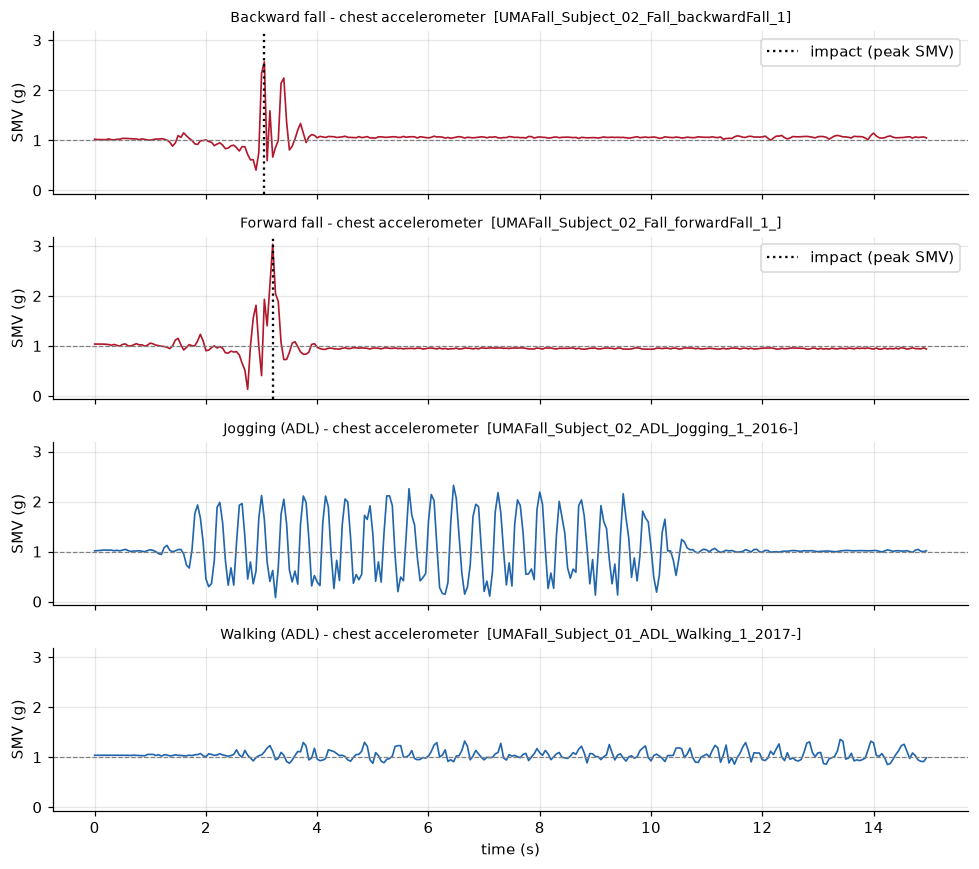
\includegraphics[width=0.78\columnwidth]{fig01_signals.png}
\caption{Chest accelerometer magnitude (SMV) in four real trials. Both falls show a dip toward 0\,g before the impact spike; jogging is repetitive and reaches a peak as large as a fall.}
\label{fig:signals}
\end{figure}

\section{Methodology}
\subsection{Preprocessing}
All sensors are brought onto a common 20\,Hz grid. The \texttt{TimeStamp} column only updates every two to three samples, so for each sensor stream we fit a straight line of timestamp against sample index and use it as a clean, evenly spaced time axis. The 200\,Hz phone signal is block-averaged (an anti-aliasing low-pass) and resampled. The magnetometer is not used. The orientation-invariant signal magnitude vector $\mathrm{SMV}=\sqrt{x^2+y^2+z^2}$ is the basis of the features, because the sensors can be rotated arbitrarily on the body. A stationary accelerometer reads about 1\,g because it senses the support force; in free fall the support vanishes and the reading approaches 0\,g, which is the physical cue that precedes the impact spike.

\subsection{Impact localisation}
For each fall trial the impact time $t_{\mathrm{imp}}$ is the time of the maximum chest SMV (waist, pocket, wrist or ankle if the chest sensor is missing). Four fall trials have a peak below 1.5\,g and the impact times range from 1.9\,s to 14.6\,s, so this definition is imperfect (Section~\ref{sec:limits}).

\subsection{Causal windows and features}
A decision at time $t$ may use only data up to $t$. We slide a 1\,s window (20 samples) over every trial, with a stride of 0.05\,s for falls and 0.1\,s for ADLs, and also use a 2\,s context. For the chest sensor this gives 133{,}957 windows. Each window yields 28 features (Table~\ref{tab:features}). The post-impact stillness that is a strong \emph{detection} feature lies in the future and is therefore excluded by design.

\begin{table}[t]
\caption{Feature groups (28 features per window)}
\label{tab:features}
\centering
\footnotesize
\begin{tabular}{@{}p{1.9cm}p{3.7cm}p{2.0cm}@{}}
\toprule
Group & Examples & Motivation \\
\midrule
Free-fall dip & min SMV, dip depth (previous mean $-$ min), share of samples $<0.7$\,g & support force vanishes \\
Dynamics & mean, std, max, range, last value, slope, jerk & sudden change \\
Orientation & tilt change between window start and end & body tips over \\
Rotation (gyro) & mean, max, std, slope, 2\,s max of angular speed & loss of balance \\
Repetitiveness & 2\,s std, peak count above 1.5\,g, mean deviation & jogging vs.\ one event \\
\bottomrule
\end{tabular}
\end{table}

\subsection{Time-to-impact labelling}
For a lead time $\tau$ the target is whether the impact will occur about $\tau$ seconds after the window ends (Fig.~\ref{fig:timeline}). A window of a fall trial is \emph{positive} if it ends in $[t_{\mathrm{imp}}-\tau-0.3\,\mathrm{s},\,t_{\mathrm{imp}}-\tau]$. It is \emph{negative} if it belongs to an ADL trial or ends more than 2\,s before the impact. Fall-trial windows in between are ambiguous and dropped, and windows after $t_{\mathrm{imp}}-\tau$ are neither trained on nor credited. With $\tau=0$ the window ends on the impact (classic detection); a larger $\tau$ forces the model to rely on the dip and tilt alone. We use nine lead times, $\tau\in\{0,0.1,0.2,0.3,0.4,0.5,0.6,0.8,1.0\}$\,s. The data are strongly imbalanced: 1{,}456 positive against 78{,}545 negative windows (about 1:54), with 53{,}956 windows ignored.

\begin{figure}[t]
\centering
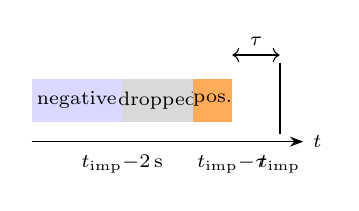
\begin{tikzpicture}[x=1cm,y=1cm,font=\scriptsize]
\fill[blue!15] (0,0) rectangle (1.15,0.55); \node at (0.575,0.275) {negative};
\fill[gray!30] (1.15,0) rectangle (2.05,0.55); \node at (1.6,0.275) {dropped};
\fill[orange!65] (2.05,0) rectangle (2.55,0.55); \node at (2.3,0.275) {pos.};
\draw[thick] (3.15,-0.15) -- (3.15,0.75);
\draw[-{Stealth}] (0,-0.25) -- (3.45,-0.25) node[right] {$t$};
\draw[<->] (2.55,0.85) -- (3.15,0.85) node[midway,above] {$\tau$};
\node[below] at (3.15,-0.3) {$t_{\mathrm{imp}}$};
\node[below] at (2.55,-0.3) {$t_{\mathrm{imp}}{-}\tau$};
\node[below] at (1.15,-0.3) {$t_{\mathrm{imp}}{-}2$\,s};
\end{tikzpicture}
\caption{Labelling for lead time $\tau$ in a fall trial (window end times). Positive windows end 0.3\,s around $t_{\mathrm{imp}}-\tau$; nothing after $t_{\mathrm{imp}}-\tau$ is used.}
\label{fig:timeline}
\end{figure}

\subsection{Models and subject-level validation}
We train a random forest (RF) \cite{breiman2001} as the main model (150 trees, minimum 5 samples per leaf, 30\% sub-sampling per tree, balanced class weights), and compare it with logistic regression on standardised features and with histogram-based gradient boosting, all from scikit-learn \cite{pedregosa2011}. Cross-validation is grouped by subject (stratified group 5-fold, seed 42): no person appears in both the training and the test part, so the model cannot memorise individuals.

\subsection{Cost-sensitive alarm threshold}
Let $C_{FN}$ be the cost of a missed fall and $C_{FP}$ the cost of a false alarm. An alarm is raised when the score exceeds a threshold $\theta$, chosen as
\begin{equation}
\theta^\star=\arg\min_{\theta}\; C_{FN}\cdot FN(\theta)+C_{FP}\cdot FP(\theta).
\end{equation}
Class weights distort the forest's probabilities, so instead of the Bayes threshold $C_{FP}/(C_{FP}+C_{FN})$ we search $\theta$ directly. To avoid leakage, $\theta^\star$ is selected on out-of-fold scores of an inner 3-fold grouped cross-validation on the \emph{training} subjects of each outer fold and then applied unchanged to the held-out subjects. The default is $C_{FN}{:}C_{FP}=10{:}1$ and is varied in Section~\ref{sec:cost}.

\subsection{Evaluation}
\emph{Window level:} ROC-AUC, PR-AUC (the more informative score at 1:54 imbalance \cite{davis2006}), recall, precision and the total cost on labelled windows. \emph{Trial level}, closer to a deployed system: a fall counts as \emph{caught} if any alarm fires on a window ending at or before $t_{\mathrm{imp}}-\tau$; for ADL trials, alarms closer than 1\,s are merged and we report alarms per minute and the share of ADL trials with at least one alarm. All scores are out-of-fold, so each subject is predicted by a model that never saw it.

\section{Results}
\subsection{Simple rules are not enough}
Single-feature rules already show the difficulty (Table~\ref{tab:baseline}). The peak SMV, the classic rule, has a ROC-AUC of only 0.65 at $\tau=0$ and 0.48 at $\tau=0.3$\,s, which is below chance. The dip and tilt features degrade more gracefully, which motivates a learned multi-feature model.

\begin{table}[t]
\caption{ROC-AUC of single-feature rules (window level)}
\label{tab:baseline}
\centering
\footnotesize
\begin{tabular}{@{}lcc@{}}
\toprule
Rule (score) & $\tau=0$ & $\tau=0.3$\,s \\
\midrule
Peak SMV (max) & 0.652 & 0.479 \\
Max jerk & 0.805 & 0.661 \\
Free-fall dip ($-$min SMV) & 0.826 & 0.759 \\
Max gyroscope & 0.864 & 0.703 \\
Tilt change & 0.868 & 0.771 \\
\bottomrule
\end{tabular}
\end{table}

\subsection{Effect of the lead time}
Table~\ref{tab:main} and Fig.~\ref{fig:tau} show the random forest on the chest sensor at the nested cost-optimal threshold. Ranking quality falls steadily: PR-AUC drops from 0.90 at impact to 0.72 at 0.3\,s, 0.33 at 0.6\,s and 0.11 at 1.0\,s. The window-level recall at the chosen threshold drops from 0.91 to 0.80, 0.57 and 0.29. At trial level, however, recall stays high (0.92--0.99 up to 0.6\,s) because a fall offers many windows in which an alarm may fire; the cost appears instead as false alarms, which rise from 1.1 to 2.8 and 5.1 per minute, and as the share of ADL trials with at least one alarm, which rises from 26\% to 55\% and 82\%. Beyond 0.8\,s the model loses on both sides (recall 0.82, then 0.64 at 1.0\,s), as the body has barely begun to lose balance. The median warning time of caught falls exceeds $\tau$ (e.g.\ 0.75\,s at $\tau=0.3$\,s) because the alarm often fires earlier than required, during the dip.

\begin{table}[t]
\caption{Random forest, chest sensor, $C_{FN}{:}C_{FP}=10{:}1$, nested threshold, subject-level 5-fold CV}
\label{tab:main}
\centering
\footnotesize
\setlength{\tabcolsep}{3.2pt}
\begin{tabular}{@{}ccccccc@{}}
\toprule
$\tau$ (s) & ROC & PR & Win.\ rec. & Falls caught & Alarms/min & ADL w/ alarm \\
\midrule
0.0 & 0.987 & 0.897 & 0.913 & 0.990 & 1.11 & 0.255 \\
0.1 & 0.978 & 0.855 & 0.863 & 0.966 & 1.49 & 0.326 \\
0.2 & 0.975 & 0.791 & 0.826 & 0.957 & 2.12 & 0.445 \\
0.3 & 0.968 & 0.722 & 0.802 & 0.942 & 2.76 & 0.549 \\
0.4 & 0.959 & 0.610 & 0.765 & 0.952 & 3.74 & 0.682 \\
0.5 & 0.940 & 0.479 & 0.720 & 0.942 & 4.76 & 0.799 \\
0.6 & 0.914 & 0.328 & 0.573 & 0.918 & 5.05 & 0.823 \\
0.8 & 0.866 & 0.169 & 0.439 & 0.822 & 5.03 & 0.810 \\
1.0 & 0.836 & 0.111 & 0.294 & 0.639 & 4.14 & 0.678 \\
\bottomrule
\end{tabular}
\end{table}

\begin{figure*}[t]
\centering
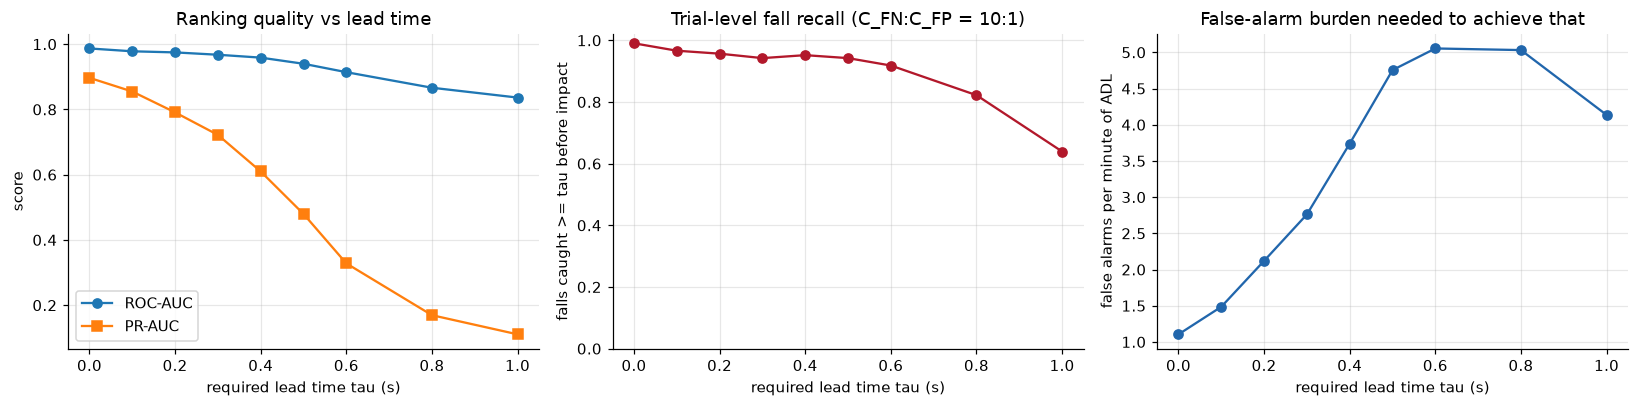
\includegraphics[width=0.95\textwidth]{fig03_tau_tradeoff.png}
\caption{Effect of the required lead time $\tau$: ranking quality (left), trial-level fall recall (middle) and false alarms per minute of daily activity (right).}
\label{fig:tau}
\end{figure*}

\subsection{Operating curves and cost sensitivity}\label{sec:cost}
Sweeping the threshold gives an operating curve per lead time (Fig.~\ref{fig:curves}); the curves sink as $\tau$ grows, i.e.\ at the same false-alarm rate fewer falls are caught early. Table~\ref{tab:cost} varies the cost ratio at $\tau=0.3$\,s. A ratio of 1:1 catches 84\% of falls at 0.7 alarms per minute, 20:1 catches 97\% at 4.4, and 100:1 catches all falls at 7.8 alarms per minute. The right ratio depends on the application: a hip airbag tolerates false alarms, a robot that stops walking does not. (In this table the threshold is tuned on the same out-of-fold scores, so it shows the shape of the trade-off rather than an unbiased estimate.)

\begin{figure}[t]
\centering
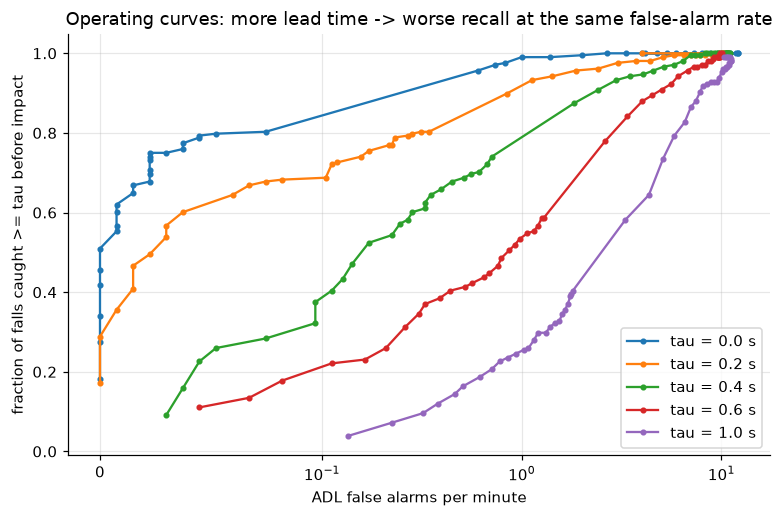
\includegraphics[width=0.82\columnwidth]{fig04_operating_curves.png}
\caption{Operating curves: share of falls caught at least $\tau$ before impact versus false alarms per minute (log-linear axis), for several lead times.}
\label{fig:curves}
\end{figure}

\begin{table}[t]
\caption{Cost-ratio sweep at $\tau=0.3$\,s (analysis; threshold tuned on out-of-fold scores)}
\label{tab:cost}
\centering
\footnotesize
\begin{tabular}{@{}ccccc@{}}
\toprule
$C_{FN}{:}C_{FP}$ & Threshold & Falls caught & Alarms/min & ADL w/ alarm \\
\midrule
1 & 0.616 & 0.837 & 0.70 & 0.168 \\
2 & 0.406 & 0.889 & 1.43 & 0.324 \\
5 & 0.283 & 0.928 & 2.08 & 0.453 \\
10 & 0.231 & 0.933 & 2.49 & 0.507 \\
20 & 0.108 & 0.971 & 4.40 & 0.732 \\
50 & 0.076 & 0.990 & 5.46 & 0.818 \\
100 & 0.036 & 1.000 & 7.76 & 0.922 \\
\bottomrule
\end{tabular}
\end{table}

\subsection{Models and important features}
At $\tau=0.3$\,s the random forest has the lowest expected cost (Table~\ref{tab:models}). Gradient boosting is close and has the higher window recall; logistic regression is clearly weaker, which indicates non-linear structure in the features. The most important random-forest features (impurity importance, trained on all data for interpretation only) are the window mean SMV (0.121), the dip depth (0.107), the minimum SMV in the last 0.5\,s (0.093) and the standard deviation of the previous second (0.093): this is consistent with a model that looks for a drop below the preceding level after a calm period.

\begin{table}[t]
\caption{Model comparison at $\tau=0.3$\,s (chest, nested threshold)}
\label{tab:models}
\centering
\footnotesize
\begin{tabular}{@{}lcccccc@{}}
\toprule
Model & ROC & PR & Rec. & Prec. & Cost & Alarms/min \\
\midrule
Logistic reg. & 0.941 & 0.472 & 0.764 & 0.328 & 5714 & 3.70 \\
Random forest & 0.968 & 0.722 & 0.802 & 0.478 & 4156 & 2.76 \\
Grad.\ boosting & 0.960 & 0.710 & 0.832 & 0.376 & 4454 & 3.95 \\
\bottomrule
\end{tabular}
\end{table}

\subsection{Sensor position}
Using accelerometer-only features, so that the gyroscope-less phone is comparable, the waist and chest placements are best (Table~\ref{tab:pos}). The pocket phone loses little (PR-AUC 0.62), which is encouraging for deployment on devices people already carry, while wrist and ankle lose most of the signal (0.28 and 0.15): limb motion is dominated by activities unrelated to falling. The waist and ankle rows use fewer trials (617 and 643), so the comparison is not perfectly paired.

\begin{table}[t]
\caption{Sensor position at $\tau=0.3$\,s (accelerometer-only features)}
\label{tab:pos}
\centering
\footnotesize
\begin{tabular}{@{}lccccc@{}}
\toprule
Position & Trials & ROC & PR & Falls caught & Alarms/min \\
\midrule
Waist & 617 & 0.974 & 0.701 & 0.989 & 3.18 \\
Chest & 745 & 0.966 & 0.698 & 0.933 & 2.85 \\
Right pocket & 746 & 0.970 & 0.623 & 0.971 & 3.74 \\
Wrist & 746 & 0.911 & 0.282 & 0.904 & 6.05 \\
Ankle & 643 & 0.904 & 0.152 & 0.847 & 4.60 \\
\bottomrule
\end{tabular}
\end{table}

\subsection{Error analysis}
At $\tau=0.3$\,s the three fall types are caught about equally often: backward 96\%, forward 94\% and lateral 92\% of trials. False alarms concentrate on activities with a rapid change of posture or a vertical impact: bending (97\% of trials with at least one alarm), lying down on a bed (81\%), jogging (79\%), hopping (77\%), sitting down and getting up (77\%) and going downstairs (75\%). Activities with little trunk motion rarely trigger alarms: making a phone call (7\%), going upstairs (15\%), raising the hands (28\%) and walking (30\%). Many of these false alarms are physically plausible, since bending and lying down also change the orientation and briefly unload the sensor.

\subsection{Strict evaluation and temporal persistence}\label{sec:ext}
The trial-level recall of Table~\ref{tab:main} credits any alarm before $t_{\mathrm{imp}}-\tau$. The \emph{strict} metric credits only alarms inside the actionable zone $[t_{\mathrm{imp}}-2\,\mathrm{s},\,t_{\mathrm{imp}}-\tau]$, and counts every alarm in the calm part of a fall trial as a false alarm (false-alarm time is ADL time plus the calm time of fall trials). We also test \emph{temporal persistence}: an alarm is raised only if the mean score over the last $\Delta$ seconds exceeds the threshold ($\Delta=0$ is the original rule; the smoothing is causal). Thresholds here are chosen on the out-of-fold scores of the other folds with the same 10:1 cost, so the $\Delta=0$ rows differ slightly from Table~\ref{tab:main}.

Table~\ref{tab:ext} shows that the strict metric lowers recall by only 2--3 points (e.g.\ 0.942 to 0.913 at $\tau=0.3$\,s), so the headline conclusions are robust to the more demanding definition. Persistence changes little at short horizons: at $\tau=0$ and 0.3\,s the false-alarm rate stays at 1.1--1.2 and 2.4--2.5 per minute while recall drops by up to 1.4 points. Only at $\tau=0.6$\,s does it help (4.91 to 3.72 alarms per minute with $\Delta=0.4$\,s, $-24\%$), at the price of 7.7 points of recall (0.894 to 0.817). Because raising the threshold alone also moves along the same trade-off curve, we cannot claim that persistence improves the operating curve; we regard it as a tunable knob and, for short horizons, a negative result.

\begin{table}[t]
\caption{Strict trial-level evaluation with temporal persistence $\Delta$}
\label{tab:ext}
\centering
\footnotesize
\begin{tabular}{@{}cccccc@{}}
\toprule
$\tau$ (s) & $\Delta$ (s) & Strict recall & Median lead (s) & Alarms/min & ADL w/ alarm \\
\midrule
0.0 & 0   & 0.971 & 0.45 & 1.21 & 0.277 \\
    & 0.2 & 0.971 & 0.40 & 1.14 & 0.263 \\
    & 0.4 & 0.962 & 0.40 & 1.21 & 0.272 \\
\midrule
0.3 & 0   & 0.913 & 0.70 & 2.46 & 0.508 \\
    & 0.2 & 0.899 & 0.65 & 2.41 & 0.490 \\
    & 0.4 & 0.899 & 0.65 & 2.48 & 0.501 \\
\midrule
0.6 & 0   & 0.894 & 1.10 & 4.91 & 0.814 \\
    & 0.2 & 0.846 & 1.05 & 4.32 & 0.771 \\
    & 0.4 & 0.817 & 1.00 & 3.72 & 0.717 \\
\bottomrule
\end{tabular}
\end{table}

\section{Discussion and Limitations}\label{sec:limits}
\textbf{Interpretation.} The lead time is not free. Each extra 100\,ms removes evidence from the window, so ranking quality falls and the threshold must be lowered to keep falls, which produces more false alarms. Around 0.2--0.4\,s the system still catches 94--96\% of falls at 2--4 alarms per minute; at 0.8\,s and beyond it cannot compensate. The fixed cost ratio is a modelling choice and should be set by the application.

\textbf{Limitations.} (i)~All falls are simulated by young, healthy volunteers; elderly falls may differ. (ii)~There are only 19 subjects and one subject contributes 56 of the 208 falls, so uncertainty is large; we report single-seed results without confidence intervals. (iii)~The 20\,Hz sampling limits the resolution of the dip to 50\,ms. (iv)~The impact time is the peak SMV, which is wrong for a few suspicious trials. (v)~The false-alarm burden is high: at $\tau=0.3$\,s, 55\% of ADL trials raise at least one alarm, so the system is not deployable as it stands. (vi)~The trial-level recall of Table~\ref{tab:main} is generous, because any alarm before $t_{\mathrm{imp}}-\tau$ counts. This explains why it exceeds the window-level recall (0.94 vs.\ 0.80 at $\tau=0.3$\,s) and why the median warning time exceeds $\tau$. The strict metric of Section~\ref{sec:ext} lowers recall by only 2--3 points. (vii)~The window-level cost used to select the threshold is a proxy for the true cost per alarm event.

\section{Conclusion}
We formulated early-warning fall prediction as a family of causal classification problems indexed by the lead time before impact, and evaluated it on UMAFall with subject-level validation and a nested cost-sensitive threshold. Falls leave an early physical signature, the free-fall dip and the tilt, which a random forest exploits: at $\tau=0.3$\,s it reaches a PR-AUC of 0.72 and catches 94\% of falls at 2.8 false alarms per minute. Demanding more lead time reduces ranking quality and mainly raises the false-alarm burden, until the evidence disappears at about 1\,s. A stricter metric changes recall by only 2--3 points, while temporal smoothing of the alarm score reduces false alarms only at the longest horizon we tested (0.6\,s) and at a cost in recall. Chest and waist sensors are most informative; the pocket phone is a practical compromise. Future work includes orientation-corrected features using the magnetometer, sequence models on the raw signals, fusion of several positions, personalised thresholds and validation on other datasets such as SisFall \cite{sucerquia2017} and, ultimately, on data from older adults. The complete code (parsing, features, models, evaluation and figures) is provided with this submission.

\begin{thebibliography}{00}
\bibitem{casilari2017} E.~Casilari, J.~A.~Santoyo-Ram\'on, and J.~M.~Cano-Garc\'ia, ``UMAFall: A multisensor dataset for the research on automatic fall detection,'' \emph{Procedia Computer Science}, vol.~110, pp.~32--39, 2017.
\bibitem{noury2007} N.~Noury \emph{et al.}, ``Fall detection -- principles and methods,'' in \emph{Proc. 29th Annu. Int. Conf. IEEE Eng. Med. Biol. Soc. (EMBC)}, Lyon, France, 2007, pp.~1663--1666.
\bibitem{igual2013} R.~Igual, C.~Medrano, and I.~Plaza, ``Challenges, issues and trends in fall detection systems,'' \emph{BioMedical Engineering OnLine}, vol.~12, art.~66, 2013.
\bibitem{elkan2001} C.~Elkan, ``The foundations of cost-sensitive learning,'' in \emph{Proc. 17th Int. Joint Conf. Artificial Intelligence (IJCAI)}, 2001, pp.~973--978.
\bibitem{breiman2001} L.~Breiman, ``Random forests,'' \emph{Machine Learning}, vol.~45, no.~1, pp.~5--32, 2001.
\bibitem{pedregosa2011} F.~Pedregosa \emph{et al.}, ``Scikit-learn: Machine learning in Python,'' \emph{J. Mach. Learn. Res.}, vol.~12, pp.~2825--2830, 2011.
\bibitem{davis2006} J.~Davis and M.~Goadrich, ``The relationship between precision-recall and ROC curves,'' in \emph{Proc. 23rd Int. Conf. Machine Learning (ICML)}, 2006, pp.~233--240.
\bibitem{sucerquia2017} A.~Sucerquia, J.~D.~L\'opez, and J.~F.~Vargas-Bonilla, ``SisFall: A fall and movement dataset,'' \emph{Sensors}, vol.~17, no.~1, art.~198, 2017.
\end{thebibliography}

\end{document}
